\documentclass[modern]{aastex631}
\bibliographystyle{aasjournal}

% \usepackage{fontspec}
% \usepackage[T1]{fontenc}
% \usepackage{newtxsf}
% \setmainfont{Fira Sans Book}[Scale=1.0]

\usepackage[caption=false]{subfig}
\usepackage{booktabs}

\begin{document}
\shorttitle{Condensate clouds with TESS and IGRINS}
\shortauthors{Gully-Santiago et al. }
\title{Disentangling brown dwarf clouds with IGRINS and contemporaneous TESS monitoring}

\author{Michael Gully-Santiago}
\affiliation{University of Texas at Austin Department of Astronomy}

\author{TBD}
\affiliation{TBD}


\begin{abstract}

We disentangle clouds on the nearby brown dwarf Luhman 16 using multi-epoch IGRINS with contemporaneous TESS monitoring.

\end{abstract}

\keywords{High resolution spectroscopy (2096)}

\section{Introduction}\label{sec:intro}

Here is an annotated bibliography.

\begin{deluxetable}{chc}
  \tablecaption{Annotated bibliography for intro\label{table1}}
  \tablehead{
  \colhead{Reference} & \nocolhead{two} & \colhead{Key idea}
  }
  \startdata
  \citet{2013ApJ...767L...1L} & - & Discovery paper\\
  \citet{2021ApJ...906...64A} & - & TESS data \\
  \citet{2016ApJ...825...90K} & - & HST Time-resolved spectroscopy maps\\
  \citet{2017MNRAS.470.1140B} & - & HST Orbit fitting\\
  \enddata
\end{deluxetable}

\section{Observations}

\subsection{IGRINS}
We acquired spectra from IGRINS \citep{park14,2018SPIE10702E..0QM} at Gemini South as part of Director's Discretionary Time proposal \texttt{GS-2021A-DD-104}.  We computed an angular separation $\rho = 1\farcs3 \pm 0 \farcs 1$ and $P.A. = 134 \pm 3^\circ$ based on the orbital parameters from Table 5 of \citet{2018A&A...618A.111L} for the epoch 2021.19; the uncertainties are based on the comparison of predictions from \citet{2017MNRAS.470.1140B} and \citet{2018A&A...618A.111L}, which came to different values at these small levels.  The $0\farcs34 \times 5\farcs0$ IGRINS slit at Gemini South presents an economic tradeoff on how to orient the slit relative to the binary.  Aligning the slit along the $P.A.$ collects more photons, but complicates the data reduction process.  Aligning the slit perpendicular to the $P.A.$ collects less flux per exposure, but allows the \texttt{plp} piepeline package \citep{jaejoonlee16} to be used for standard and well-tested data reduction.  We chose the latter strategy, aligning the IGRINS $P.A.$ to $44^\circ$, as shown in Figure \ref{fig:imaging}.



Luhman~16 appears near a local maximum of projected sky separation in 2021, with the B component expected to reside South and East of the A component.

\begin{figure*}[ht]
  \centering
    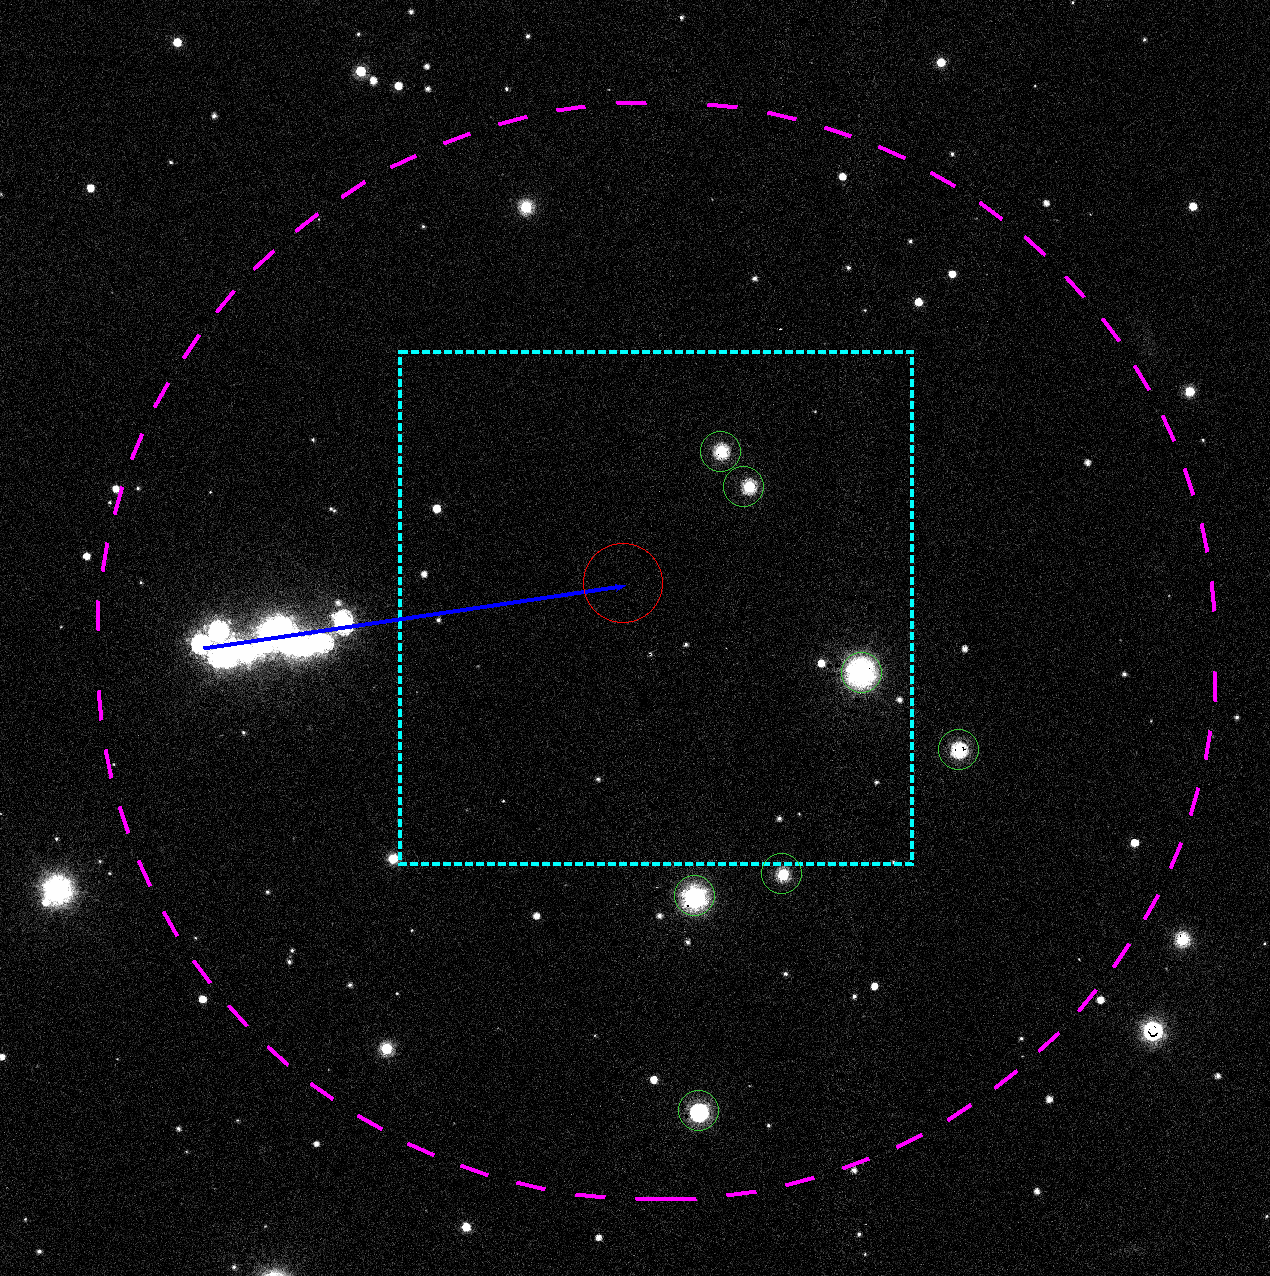
\includegraphics[width=1.9in]{figures/DS9_HST_zoom_in_matched.png}
    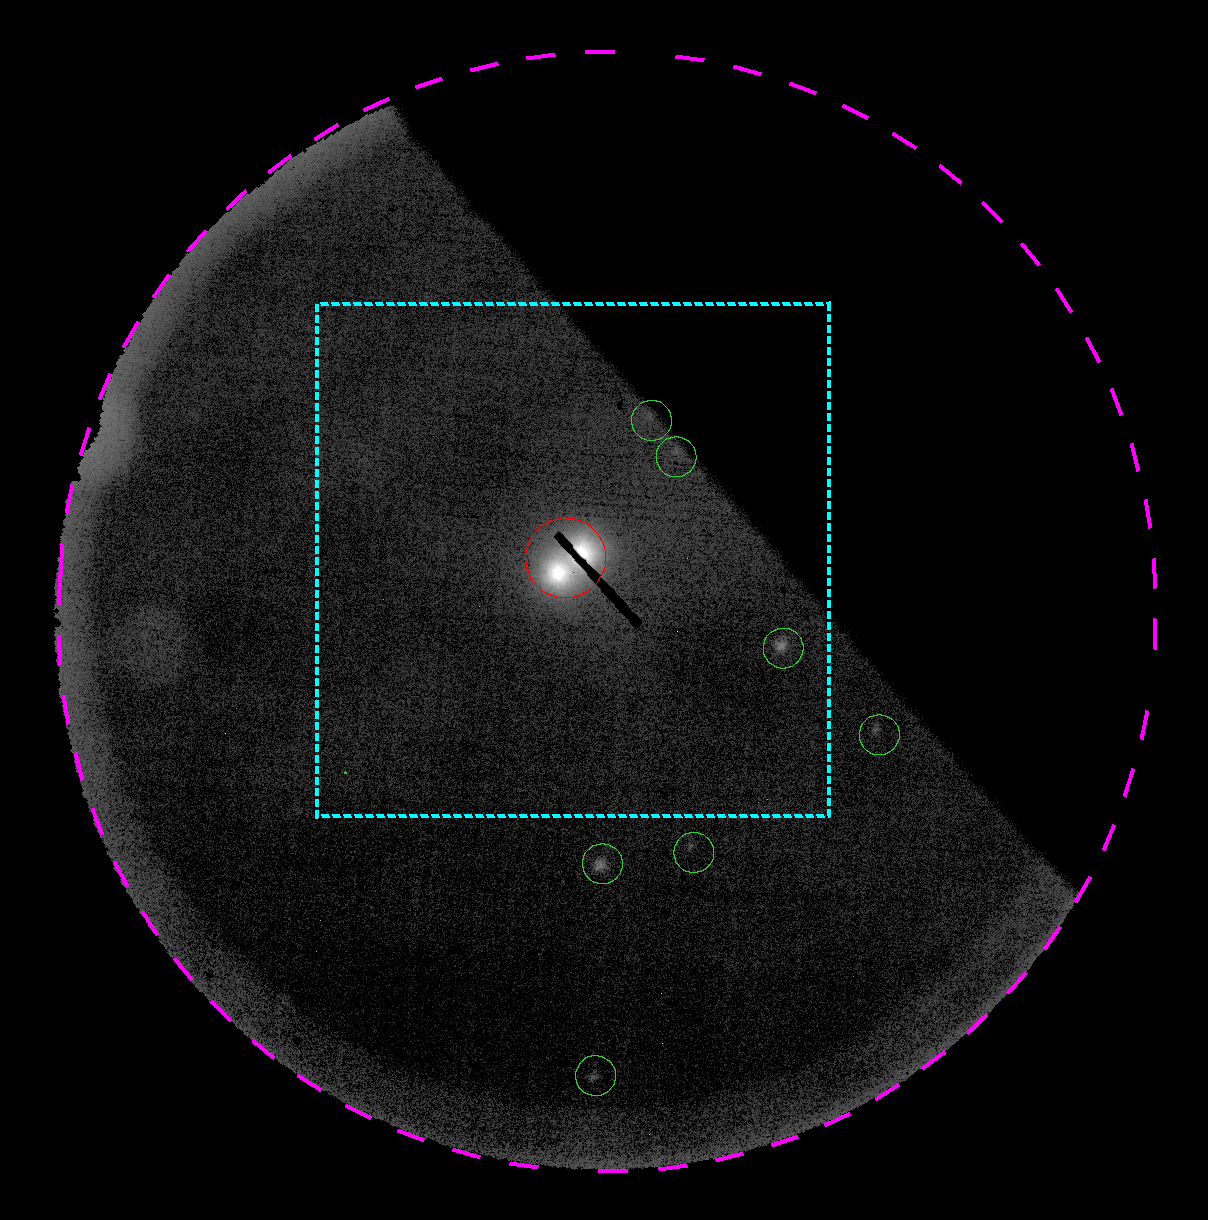
\includegraphics[width=1.9in]{figures/DS9_IGRINS_SVC_zoom_in.png} \\
\caption{Imaging of Luhman~16, with North up and East to the left.  \texttt{Left:} \emph{Hubble Space Telescope} WFC3/UVIS/F814W mosaic from 12 visits of in 2014.638 to 2016.757 \citep{2017MNRAS.470.1140B}.  The thin blue line illustrates the approximate path of the proper motion, with a thin red circle denoting the binary's approximate expected position for 2021. A $21'' \times 21''$ postage stamp---equal to the size of one TESS pixel---appears as a dashed cyan square.  \texttt{Right:} The IGRINS $K-$band Slit Viewing Camera (SVC) at Gemini South on March 11, 2021.  The expected P.A. of the AB components was intentionally aligned perpendicular to the $0\farcs34 \times 5\farcs0$ IGRINS slit, seen as a black diagonal silhouette. Seven faint background reference stars common to both images are circled in green.  TESS Full Frame Images (not shown) and resulting lightcurves consist of the integrated light from both components.  The A component is to the northwest (upper right) with the B component to the southeast (lower left).  The magenta dashed circle shows the extent of the (vignetted) SVC.}
\label{fig:imaging}
\end{figure*}


%\begin{figure*}[ht]
%  \centering
%    \includegraphics[width=3in]{figures/Luhman16_IGRINS_slit_20210311.pdf} \\
%\caption{A $21'' \times 21''$ postage stamp---equal to the size of one TESS pixel---of the IGRINS $K-$band Slit Viewing Camera at Gemini South on March 11, 2021.  The color scale is inverted.  The PA of the AB components was intentionally aligned perpendicular to the $0\farcs34 \times 5\farcs0$ IGRINS slit seen as a white diagonal silhouette to the southeast (bottom left) of the binary. TESS Full Frame Images (not shown) and resulting lightcurves consist of the integrated light from both components.}
%\label{fig:imaging}
%\end{figure*}

Table \ref{table1} lists the BTJD of each binary component on each night.

\begin{deluxetable}{ccc}
  \tablecaption{IGRINS Observing Log\label{table1}}
  \tablehead{
    \colhead{Night of} & \colhead{Bin. Comp.} &\colhead{BTJD}}
  \startdata
  \input{IGRINS_obs_log.txt}
  \enddata

\end{deluxetable}

\section{Analysis}

\subsection{TESS lightcurves}

TESS observed Luhman~16 in Sectors 36 and 37 with 10-minute cadence in the Full-Frame Images (FFI).  It was not preselected for 2-minute or shorter cadences.  For Sector 36, we retrieved $3477$ calibrated, Early Release Full Frame Image TICA products \citep{2020RNAAS...4..251F} from \emph {TESS} Camera 3 CCD 1, hosted on \emph{MAST}.  We extracted $17$-pixel square postage stamps centered on the expected $x,y$ coordinates of Luhman~16 $(538, 155)$, discarding the rest of the voluminous FFI.  We assigned a 2- to 4-pixel target aperture based on those central pixels routinely exceeding a threshold above the median of the $17\times17\times3477$ datacube. We constructed a non-contiguous 68-pixel background mask of those pixels in the bottom $15^{th}$ percentile of a median-combined-flux image and greater than 15 pixels away from the postage-stamp center position. The background-subtracted lightcurve was trimmed to remove portions of the data degraded by thermal settling immediately after data downlinks and fine-point acquisition.  We also removed conspicuous outliers 3 standard deviations above or below the median flux.  The final Sector 36 flux time-series contained 3087 time-points.  We adapted the same process for Camera 3 CCD 2 in Sector 37, yielding a 23.7-day lightcurve of 3109 time-points.  The two lightcurves were normalized to their median value.  No attempt was made to vertically register the two lightcurves.

We also extracted the Sector 10 30-minute cadence lightcurve using a similar methodology, adapted in the following way.  We retrieved a sequence of $16\times51$ TESS FFI cutouts as a Target Pixel File (TPF) using the \emph{TESScut} tool hosted on \emph{MAST}.  We used a 4-pixel target aperture and tolerated background pixels at any separation from the target.  The final Sector 10 lightcurve possessed 971 time points spanning 23.6 days.

The Sector 10, 36, and 37 lightcurves are shown in Figures XX, \ref{fig:Sector36}, and ZZ.  Figure \ref{fig:Sector36} indicates the acquisition times of the contemporaneous IGRINS spectroscopy.  The reduced TESS lightcurves, IGRINS data, and reproducible reduction scripts are publicly available\footnote{\url{https://github.com/BrownDwarf/varsity}}.

\begin{figure*}[ht]
  \centering
    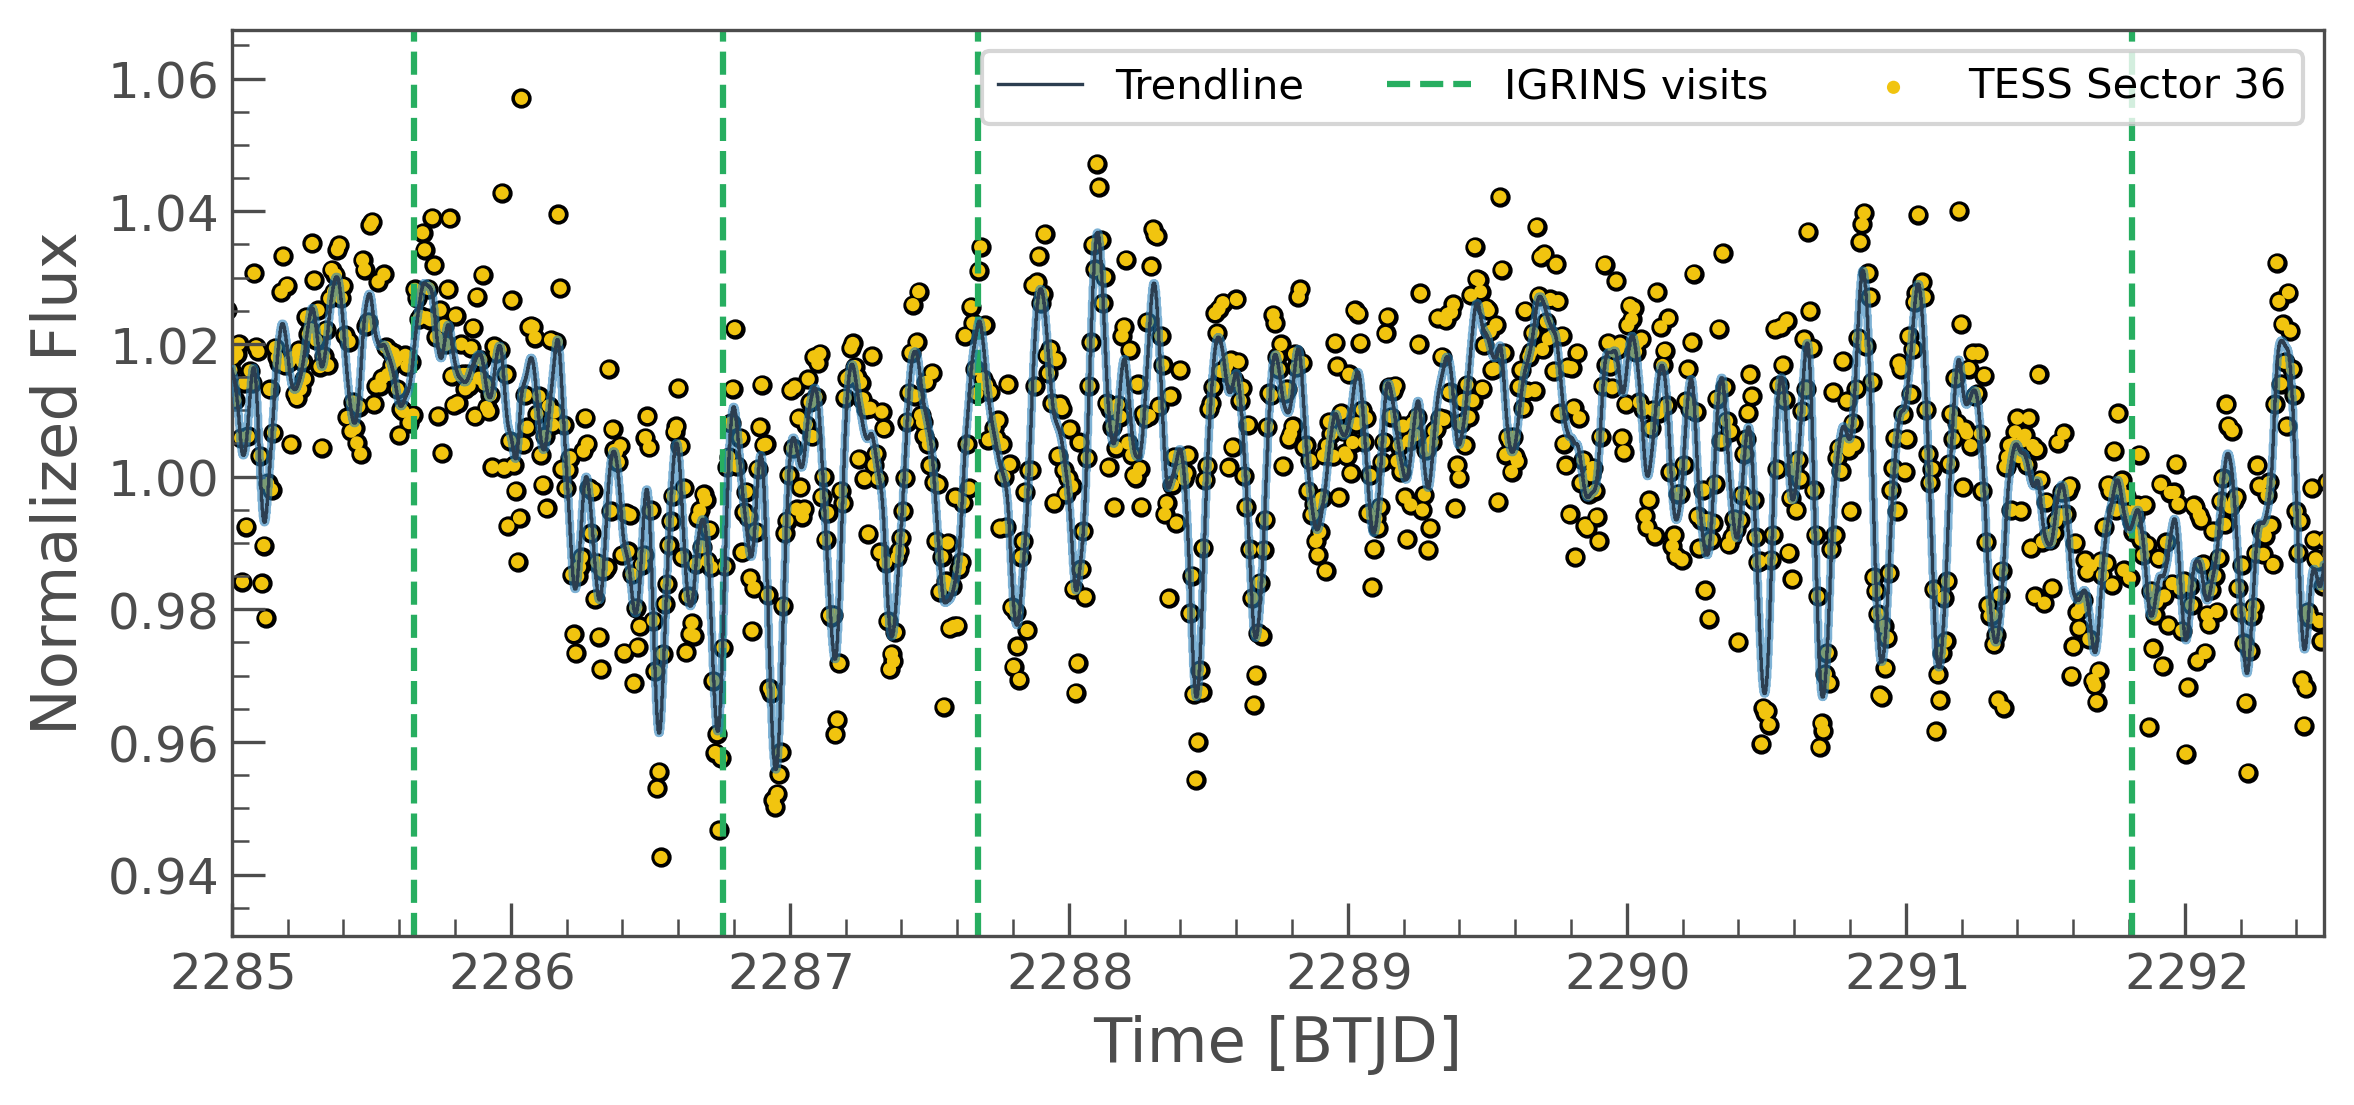
\includegraphics[width=\textwidth]{figures/TESS_S36_O1_IGRINS_overlay.png} \\
\caption{\emph{TESS} Sector 36 lightcurve of Luhman~16AB showing epochs of IGRINS visits.}
\label{fig:Sector36}
\end{figure*}

Figure ZZ overplots the Sector 10 \texttt{PATHOS} lightcurve of \citet{2021ApJ...906...64A} with our custom reduction.  We see excellent agreement between the two methods.  Our approach apparently offers a more stable lightcurve during the thermal settling windows, with recovery of up to $10\%$ additional time-points residing near the mean-line trend.

\subsection{Digitized Photographic Plates}
We attempted to recover the position of Luhman~16 from historical photographic plates recently digitized through the \emph{DASCH} project citeXX.  We retrieved a sequence of 34 thumbnails spanning 1926 - 1952.  We matched a constellation of 11 conspicuous stars in the \emph{HST} imaging from \citet{2017MNRAS.470.1140B} (c.f. Figure \ref{fig:imaging}), with each star comparable in magnitude to Luhman~16.  The constellation pattern was barely perceptible in the DASCH images.  An animated sequence of the images yielded no detectable movement in the vicinity of Luhman~16's expected proper motion path.  This non-detection comports with the faint visible band flux of Luhman~16 and the limiting magnitude of $12-14$ for \emph{DASCH}.

\subsection{Estimates for cloud properties}

\begin{figure*}[ht]
  \centering
    \includegraphics[width=\textwidth]{figures/IGRINS_low_resolution_T_bright_labeled.png} \\
\caption{Brightness temperature in the $H-$ and $K-$ bands for an $f_{\mathrm{sed}}=2$, $T_{\mathrm{eff}}=1300\;$K m demarcated with the \emph{IGRINS} \'echelle order boundaries from $m=125$ to $m=71$.  The peak of the $H-$band probes the deepest and therefore hottest region}
\label{fig:brightness_temp}
\end{figure*}

\section{Results}
State the discoveries here.

\section{Discussion}

\subsection{Future IGRINS observation strategies}
Luhman~16 will remain a benchmark target for the forseeable future, with hundreds more hours of valuable telescope resources plausibly destined for this single target.  Here we examine the tradeoffs in how future observation strategies could make the most judicious use of scarce resources moving forward.

Things to say:  
\begin{enumerate}
  \item Slit alignment: How does alignment change with orbital separation  
  \item The limits on the ability to calibrate the relative fluxes on the same slit  
  \item Slit alignment: How the uncertainty in the orbital projection flows down to alignment  
  \item The technical barrier of extracting two traces from the same echellogram, sky subtraction and PSF fitting (spectroastrometry)  
  \item Point-and-stare versus snapshots and night-to-night calibration 
  \item PSF Decomposition on the slit  
\end{enumerate}

\subsection{Future TESS observation strategies}
\begin{enumerate}
  \item Should it receive 2-minute or shorted cadence in the future? 
  \item Strategies for contemporaneous observations: spectra in the same band?  
  \item Contemporaneous Panchromatic spectra or some sparse ground-based R-band photometry or spectrophotometry?
\end{enumerate}


\begin{acknowledgements}
Based on observations obtained at the international Gemini Observatory, a program of NSF’s NOIRLab, which is managed by the Association of Universities for Research in Astronomy (AURA) under a cooperative agreement with the National Science Foundation. on behalf of the Gemini Observatory partnership: the National Science Foundation (United States), National Research Council (Canada), Agencia Nacional de Investigaci\'{o}n y Desarrollo (Chile), Ministerio de Ciencia, Tecnolog\'{i}a e Innovaci\'{o}n (Argentina), Minist\'{e}rio da Ci\^{e}ncia, Tecnologia, Inova\c{c}\~{o}es e Comunica\c{c}\~{o}es (Brazil), and Korea Astronomy and Space Science Institute (Republic of Korea).

This work used the Immersion Grating Infrared Spectrometer (IGRINS) that was developed under a collaboration between the University of Texas at Austin and the Korea Astronomy and Space Science Institute (KASI) with the financial support of the Mt. Cuba Astronomical Foundation, of the US National Science Foundation under grants AST-1229522 and AST-1702267, of the McDonald Observatory of the University of Texas at Austin, of the Korean GMT Project of KASI, and Gemini Observatory.

This paper includes data collected by the TESS mission. Funding for the TESS mission is provided by the NASA's Science Mission Directorate.

This paper includes analysis on data from the DASCH project at Harvard (NSF grants AST-0407380, AST-0909073, and AST-1313370).

The authors acknowledge the Texas Advanced Computing Center (TACC, \url{http://www.tacc.utexas.edu}) at The University of Texas at Austin for providing HPC resources that have contributed to the research results reported within this paper.
\end{acknowledgements}

\clearpage


\facilities{Gemini South (IGRINS), TESS, DASCH}

\software{  pandas \citep{mckinney10, reback2020pandas},
  emcee \citep{foreman13},
  matplotlib \citep{hunter07},
  astroplan \citep{astroplan2018},
  astropy \citep{exoplanet:astropy13,exoplanet:astropy18},
  exoplanet \citep{exoplanet:exoplanet},
  numpy \citep{harris2020array},
  scipy \citep{jones01},
  ipython \citep{perez07},
  starfish \citep{czekala15},
  bokeh \citep{bokehcite},
  seaborn \citep{waskom14}}
  %pytorch \citep{NEURIPS2019_9015}} % No pytorch yet!


\bibliography{ms}


\clearpage

\appendix
\restartappendixnumbering

\section{Assumptions about cloud spectra} \label{appendix:clouds}

Here are some more details about how we describe clouds.
\end{document}
